\documentclass[tikz,border=2pt]{standalone}
\usepackage{amsmath,amssymb}
\usepackage{tikz}

\begin{document}
% Pairing the four odd-degree vertices of a street network: the three perfect matchings have
% costs 9, 11 and 13 (shortest-path distances); the cheapest pairing is added to make the
% network Eulerian.
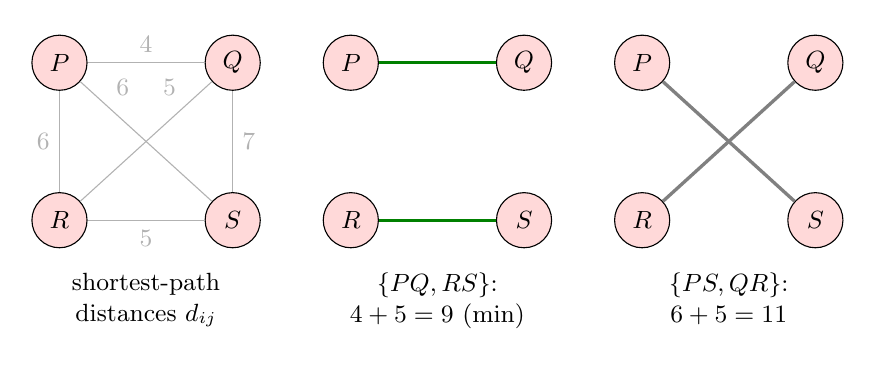
\begin{tikzpicture}[every node/.style={font=\small}, v/.style={draw, circle, fill=red!15, minimum size=7mm, inner sep=0pt}]
	\begin{scope}
		\node[v] (P) at (0,2) {$P$}; \node[v] (Q) at (2.2,2) {$Q$}; \node[v] (R) at (0,0) {$R$}; \node[v] (S) at (2.2,0) {$S$};
		\draw[gray!60] (P) -- (Q) node[midway, above] {$4$};
		\draw[gray!60] (R) -- (S) node[midway, below] {$5$};
		\draw[gray!60] (P) -- (R) node[midway, left] {$6$};
		\draw[gray!60] (Q) -- (S) node[midway, right] {$7$};
		\draw[gray!60] (P) -- (S) node[pos=0.2, above right] {$6$};
		\draw[gray!60] (Q) -- (R) node[pos=0.2, above left] {$5$};
		\node[anchor=north, align=center] at (1.1,-0.55) {shortest-path\\ distances $d_{ij}$};
	\end{scope}
	\begin{scope}[xshift=3.7cm]
		\node[v] (P) at (0,2) {$P$}; \node[v] (Q) at (2.2,2) {$Q$}; \node[v] (R) at (0,0) {$R$}; \node[v] (S) at (2.2,0) {$S$};
		\draw[green!50!black, very thick] (P) -- (Q); \draw[green!50!black, very thick] (R) -- (S);
		\node[anchor=north, align=center] at (1.1,-0.55) {$\{PQ,RS\}$:\\ $4+5=9$ (min)};
	\end{scope}
	\begin{scope}[xshift=7.4cm]
		\node[v] (P) at (0,2) {$P$}; \node[v] (Q) at (2.2,2) {$Q$}; \node[v] (R) at (0,0) {$R$}; \node[v] (S) at (2.2,0) {$S$};
		\draw[gray, very thick] (P) -- (S); \draw[gray, very thick] (Q) -- (R);
		\node[anchor=north, align=center] at (1.1,-0.55) {$\{PS,QR\}$:\\ $6+5=11$};
	\end{scope}
	\end{tikzpicture}
\end{document}
